\question{Газовые лазеры. Лазеры на СО}
Генерация осуществляется на колебательно-вращательных переходах в основном 
электронном состоянии молекулы \( CO \). Длина волны заключена в интервале 
5-6,5 мкм. Колебательное возбуждение происходит путём непосредственного 
заселения высших колебательных уровней молекулы \( CO \) при столкновениях с 
электронами газового разряда, при переходе от колебательно-возбуждённых 
молекул \( N_2 \) или ещё как-нибудь. В этом смысле этот лазер подобен 
\( CO_2 \)-лазеру.

Молекула \( CO \) является существенно ангармоническим осциллятором, поэтому 
полная колебательная инверсия отсутствует (что это значит?). В распределении 
населённостей по колебательным уровням наблюдается плато, то есть населённости 
нескольких колебательных уровней приблизительно равны.

\begin{figure}[h]
    \center
    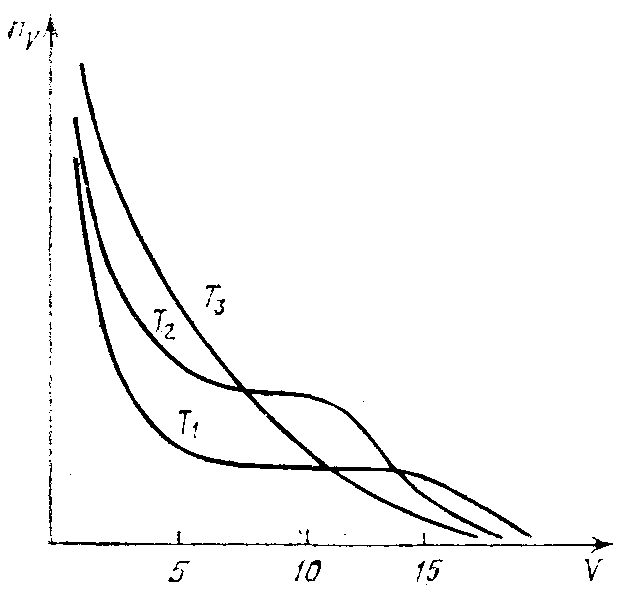
\includegraphics[width=.47\textwidth]{23_1}\hfill
    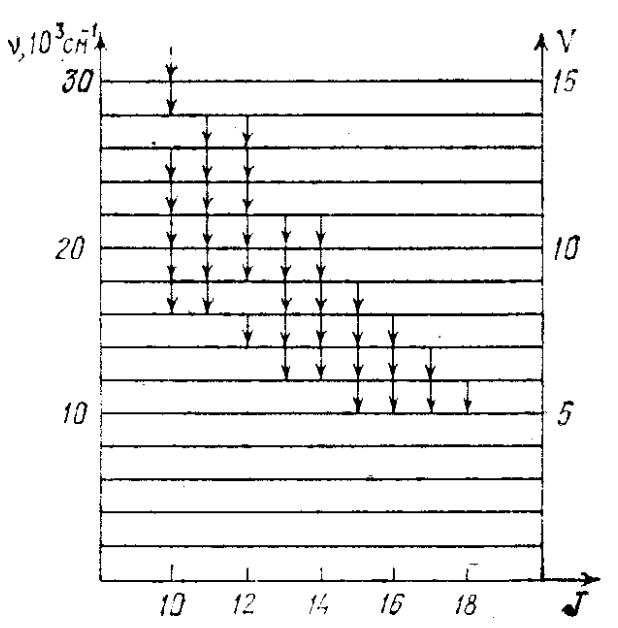
\includegraphics[width=.47\textwidth]{23_2}
    \parbox[t]{.47\textwidth}{\caption{Уровни энергии молекулы \( CO \)}}\hfill
    \parbox[t]{.47\textwidth}{\caption{Каскадные переходы}}
\end{figure}

Найдите где-нибудь нормальное описание процессов в этом лазере.

Суммарный по всем линиям генерации КПД может достигать весьма больших 
значений. Возможна работа в импульсном и непрерывном режимах. Применение в 
качестве буферного газа ксенона позволяет перейти к комнатной температуре и 
отпаянным системам. Характерной особенностью этого лазера является отсутствие 
колебательной инверсии и каскадный характер генерации в \( P \)-ветви 
колебательно-вращательных переходов.